
\documentclass[10pt]{beamer}
\usepackage{kotex}

\usepackage{framed}
\usepackage{graphicx}
%https://www.overleaf.com/learn/latex/Inserting_Images

\usepackage{amsmath}
%use dfrac
\usepackage{xcolor}

\usepackage{amsthm}
%\usepackage{tabl}
\usepackage{listings}
\definecolor{mGreen}{rgb}{0,0.6,0}
\definecolor{mGray}{rgb}{0.5,0.5,0.5}
\definecolor{mPurple}{rgb}{0.58,0,0.82}
\definecolor{backgroundColour}{rgb}{0.95,0.95,0.92}
%https://tex.stackexchange.com/questions/348651/c-code-to-add-in-the-document
\lstdefinestyle{CppStyle}{
    backgroundcolor=\color{backgroundColour},   
    commentstyle=\color{mGreen},
    keywordstyle=\color{magenta},
    numberstyle=\tiny\color{mGray},
    stringstyle=\color{mPurple},
    basicstyle=\footnotesize,
    breakatwhitespace=false,         
    breaklines=true,                 
    captionpos=b,                    
    keepspaces=true,                 
    numbers=left,                    
    numbersep=5pt,                  
    showspaces=false,                
    showstringspaces=false,
    showtabs=false,                  
    tabsize=2,
    language=C++
}

\usepackage{url}

\usepackage{etoolbox}
\AtBeginEnvironment{quote}{\singlespacing\small}


\usepackage{thmtools}
\usepackage{xcolor}
\declaretheoremstyle[% spaceabove=6pt,spacebelow=6pt, headfont=\color{MainColorOne}\sffamily\bfseries, notefont=\mdseries, notebraces={[}{]}, bodyfont=\normalfont,
headpunct={},
postheadspace=1em,
%qed=▣,
]{maintheorem}

\declaretheorem[%
name=정의,
style=maintheorem,
numberwithin=section, shaded={%bgcolor=MainColorThree!20,
margin=.5em}]{dfn}
% \begin{dfn}[]
% \end{dfn}

\setbeamertemplate{footline}[frame number]

%\usetheme{Hannover}
\usetheme{CambridgeUS}


\title{분할정복}

\author{EUnS}

\begin{document}


\begin{frame}{}
    \maketitle
\end{frame}    

% \begin{frame}{}
%     \tableofcontents
% \end{frame}   




\begin{frame}{merge sort}
    \href{https://www.youtube.com/watch?v=2YvFRAC8UTM&list=PL52K_8WQO5oUuH06MLOrah4h05TZ4n38l&index=11&t=0s}{\textcolor{blue}{참고}}
    \begin{itemize}
        \item $\Theta(n\lg n)$
        \item 분할 : 정렬할 n개의 원소의 배열을 $n/2$개씩 부분 수열 두 개로 분할한다.
        \item 정복 : 두 부분 배열을 재귀적으로 정렬한다.
        \item 결합: 정렬된 두 개의 부분 배열을 병합해 정렬된 배열 하나로 만든다.
    \end{itemize}
\end{frame}



\begin{frame}{}
    \begin{figure}[h!]
        %\centering
        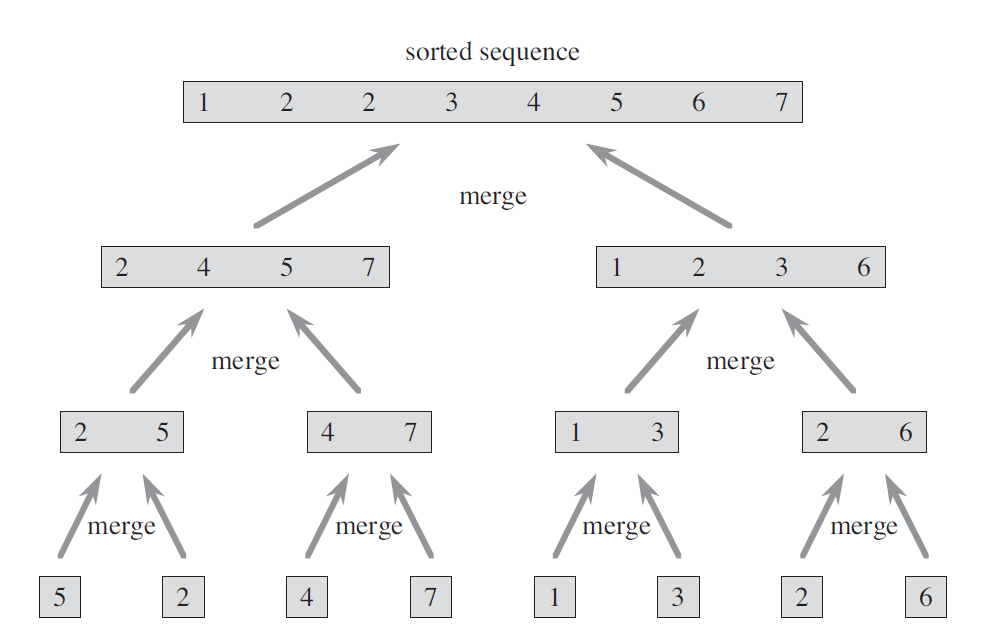
\includegraphics[scale=0.4]{merge.png}
        %\caption{}
    \end{figure}
\end{frame}    




\begin{frame}[fragile]{}
        
    \begin{lstlisting}[style = CppStyle]
    MERGE(A, p, q, r)
        n1 = q - p + 1
        n2 = r - q
        let L[1...n1 + ] and R[1..n2 + 1] be new arrays
        for i = 1 to n1
            L[E] = A[p + i - 1]
        for j = 1 to n2
            R[j] = A[q + j]
        L[n1 + 1] = INF
        R[n2 + 1] = INF
        i = 1
        j = 1
        for k = p to r
            if L[i] <= R[j]
                A[k] = L[i]
                i = i + 1
        else 
            A[E] = R[j]
            j = j + 1
    \end{lstlisting}

\end{frame}    

\begin{frame}[fragile]{}
    \begin{lstlisting}[style = CppStyle]
    MERGE-SORT(A, p, r)
        if p < r
            q = (p + r)/2
            MERGE-SORT(A, p, q)
            MERGE-SORT(A, q + 1, r)
            MERGE(A, p, q, r)
    \end{lstlisting}
\end{frame}    



\begin{frame}{점화식}

    \begin{itemize}
        \item 상수 $c$보다 작은 $n$에 대해 해를 직접 구하면 상수시간에 풀수있는경우. $\Theta(1)$
        \item 주어진 문제를 문제의 $1/b$인 $a$개의 문제로 분할 하는경우 : $aT(n/b)$
        \item 분할 : $D(n)$
        \item 결합 : $C(n)$
    \end{itemize}

    \[
        T(n) = 
    \begin{cases}
        \Theta(1) (\mbox{if  } n \le c)\\
        aT(n/b) + D(n) + C(n) (\mbox{otherwise})
    \end{cases}    
    \]
\end{frame}


\begin{frame}{머지소트 점화식}

    \begin{itemize}
        \item 분할 : $D(n) = \Theta(1)$
        \item 정복 : $2T(n/2)$
        \item 결합 : $C(n) = \Theta(n)$
    \end{itemize}

    \[
        T(n) = 
    \begin{cases}
        \Theta(1) (\mbox{if  } n = 1)\\
        2T(n/2) + \Theta(n) (\mbox{if    } n > 1)
    \end{cases}    
    \]
\end{frame}




\begin{frame}{점화식 풀이법}
    \begin{itemize}
        \item 재귀 트리 방법(recursion tree method)
        \item 치환법(substitution method)
        \item 마스터 방법(master method)
    \end{itemize}
\end{frame}



\begin{frame}{재귀 트리 방법}
    \begin{figure}[h!]
        %\centering
        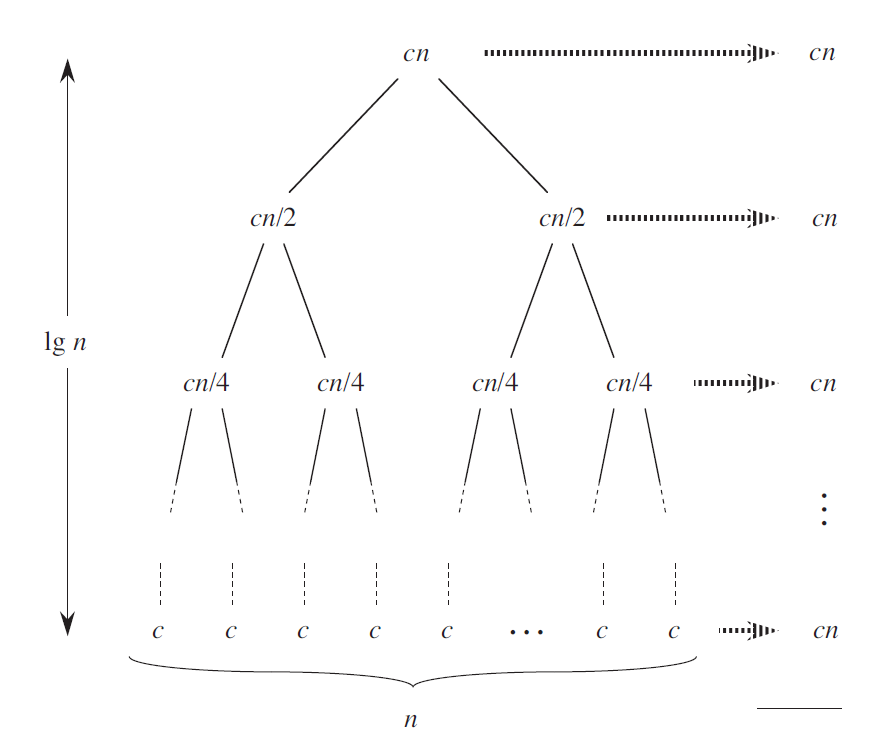
\includegraphics[scale=0.4]{mergetree.png}
    \end{figure}
\end{frame}    




\begin{frame}{재귀 트리 방법}
    $$\Theta(n \lg n)$$
\end{frame}


\begin{frame}{ex}
    $T(n) = 3T(n/4) + \Theta)n^2$
    
    \begin{figure}[h!]
        %\centering
        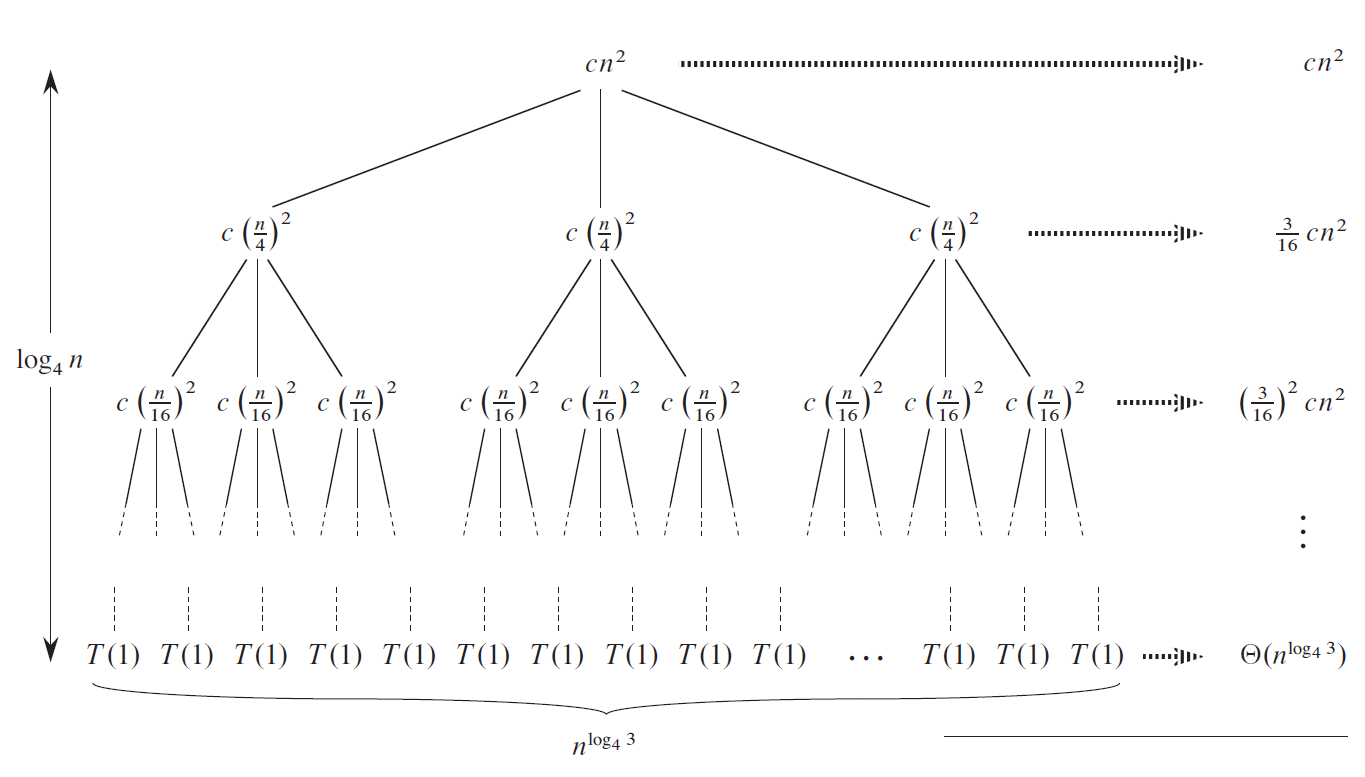
\includegraphics[scale=0.3]{tree.png}
    \end{figure}
\end{frame}


\begin{frame}[fragile]{풀이}
    \[
        \begin{aligned}
            T(n) &= \sum_{i=0}^{\log_4 n-1} \left( \dfrac{3}{16} \right)  ^i cn^2 + \Theta(n^{\log_4 3}) \\
            &<  \sum_{i=0}^{\infty} \left( \dfrac{3}{16} \right)^i cn^2 + \Theta(n^{\log_4 3}) \\
            &= \dfrac{1}{1-(3/16)}cn^2 + \Theta(n^{\log_4 3})\\
            &= O(n^2)
        \end{aligned}
    \]
\end{frame}

\end{document}



% \begin{frame}[fragile]{}
        
%     \begin{lstlisting}[style = CppStyle]
    
%     \end{lstlisting}

% \end{frame}    
% \stop


% \begin{frame}{$O$}
%     \begin{itemize}
%         \item 
%         \item 
%         \item 
%     \end{itemize}
% \end{frame}


% \begin{frame}{}
%     \href{}{\textcolor{blue}{참고}}
% \end{frame}    
